\scanpage{19}
\figure{\begin{tikzpicture}\draw (0,0)--(-.03,.8);\end{tikzpicture}}
\uline{Th. de préparation ``formel''} Soit $A$ un anneau linéairement topologique, séparé et complet, $Z$ une indéterminée,
\[
F\deleted{(\unsure{Z})}=\sum_{i\geq0}a_iZ^i\in A[[Z]],\quad N\in\mathbb N\text{ tel que}
\]
i) $a_i$ est top.$^t$ nilpotent pour $0\leq i\leq N-1$

ii) $a_N$ est inversible

Alors $F$ est un élément régulier de $A[[Z]]$ et $A[[Z]]/F$ a comme base $(Z^i)_{0\leq i\leq N-1}$, en d'autres termes tout élément $G$ de $A[[Z]]$ se met de façon unique sous la forme
\[
G=QF+\sum_{0\leq i\leq N-1}b_iZ^i\qquad
\begin{array}{l}Q\in A[[Z]]\\b_i\in A.\end{array}
\]

\figure{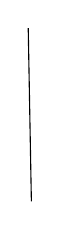
\begin{tikzpicture}\draw (0,0)--(-.04,2.2);\end{tikzpicture}}

\uline{Démonstration} Comme $A$ est séparé et complet pour sa top. linéaire, on est ramené aussitôt au cas où $A$ est discret, alors i) signifie que les $a_i$ ($0\leq i\leq\unsure{n|N}-1$) sont top. nilpotents. Soit $\mathfrak m$ l'idéal \inserted{(nilpotent)} qu'ils engendrent, $A_0=A/\mathfrak m$, et désignons par $\dot a_i,\dot F$ etc les réductions mod $\mathfrak m$. \deleted{\unsure{Alors}} Donc on a \deleted{$\unsure{\dot a}$}
\[
\dot a_i=0\quad\text{pour }0\leq i\leq N-1
\]
i.e.
\[
\dot F=\dot a_{N\deleted{\unsure{n}}}Z^{N\deleted{\unsure{n}}}+\cdots
=\dot a_{N\deleted{\unsure{n}}}Z^{N\deleted{\unsure{n}}}(1+\cdots)
\]
donc, comme $\dot a_{N\deleted{\unsure{n}}}$ est inversible par (ii), on voit que $\dot F$ est de la forme
\[
\dot F=\dot U Z^N.
\]
\deleted{\unsure{On voit donc}} donc
\[
\unsure{\dot A_0|A_0}[[Z]]/\dot F=A_0[[Z]]/Z^N\deleted{=A_0[Z]/Z^{\unsure{n|N}}}
\]
a comme base les $Z^i$ ($0\leq i\leq N-1$)

i.e.
\deleted{i) les $Z^i$ ($0\leq i\leq N-1$) engendrent $A[[Z]]/FA[[Z]]$.

En effet, ils engendrent mod $\mathfrak m$, on gagne donc par Nakayama.
\deleted{\unsure{Remarquons que}} \inserted{\unsure{le gr. associé de}} $A[[Z]]$ filtré $\mathfrak m$-adiquement \deleted{\unsure{par une}} \unsure{l'idéal}.

ii) $F$ est régulier. En effet, \unsure{a un gr. associé isomorphe à} $\unsure{\operatorname{Gr}_{\mathfrak m}^*(A)^{\mathbb N}|\operatorname{Gr}_{\mathfrak m}^*(A)[[Z]]}$.
\deleted{\unsure{de la nilpotence de} $\mathfrak m$, SPS $\mathfrak m=0$. Soit $Q\in A[[Z]]/\mathfrak m$ tel que $QF=0$, donc $\unsure{Q=0}$.}
Et l'opération de multiplication par $F$ dessus, sur le gradué associé: l'op. de multiplication par $\dot F$, qui est injective, OK.}
\figure{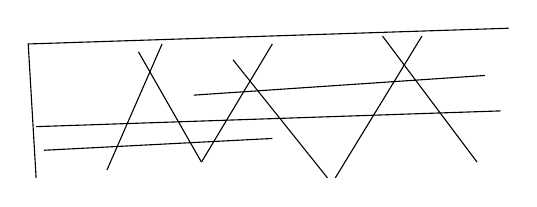
\begin{tikzpicture}[x=1cm,y=1cm]\draw (0,0)--(-.1,1.7)--(6,1.9);\draw (1.3,1.6)--(2.1,.2);\draw (1.6,1.7)--(.9,.1);\draw (2.5,1.5)--(3.7,0);\draw (3,1.7)--(2.1,.2);\draw (4.4,1.8)--(5.6,.2);\draw (4.9,1.8)--(3.8,0);\draw (2,1.05)--(5.7,1.3);\draw (0,.65)--(5.9,.85);\draw (.1,.35)--(3,.5);\end{tikzpicture}}
\mspage{18}
